% \subsection{Physical limits with ``fair'' queuing}
% \label{sec:queuing}

% However, this limitation approach does not attempt to utilize data plane performance knowledge (i.e., Interest satisfaction ratio statistics) to discriminate good and malicious Interests.

To partially overcome deficiencies of the Physical limits algorithm we need to ensure that the forwarded Interests represent at least a ``fair'' mix of the Interests received from different neighbors (interfaces).
That is, if the routers A on Fig.~\ref{fig:flooding example} has a very tight token budget, these tokens should be fairly distributed between incoming interfaces \texttt{eth0} and \texttt{eth1}.
Because of the very small volume of Interests, we cannot simply rely on network buffers to do statistical multiplexing of Interests, as they would almost never be buffered.
At the same time, until bag of tokens is not empty, there is no reason to delay Interest forwarding, as we do not known how many and from which interfaces Interests will arrive in the future.
Therefore, in order to achieve the goal of ``fair'' mixing of Interests, we need to implement additional mechanisms to buffer and mix incoming Interests, only if they cannot be immediately forwarded.

For the buffering part, we can reuse Pending Interest Table, with a small extension to support flagging of the Interests that cannot be forwarded immediately (see example on Fig.~\ref{fig:queueing}). 
As for the mixing part, we need an additional fair queuing mechanism, which can be implemented in a form of hierarchical queues (on Fig.~\ref{fig:queueing})\footnote{This essentially is a class based queuing, with classes for each outgoing/incoming interface.} or using virtual time approach~\cite{zhang1990virtual}. 
It should be noted that unlike normal queuing, Interest queues do not actually store a packet, but merely a bi-directional pointer to the existing PIT entry.
This way, PIT entry can be quickly updated when the Interest is actually forwarded, as well as the element can be removed from the queue when the Interest expires.

\begin{figure}[htbp]
  \centering
  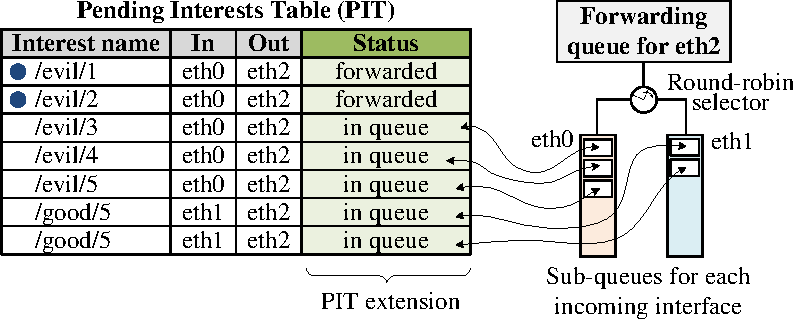
\includegraphics[scale=0.65]{queue}
  \caption{Interest queuing: if tokens are unavailable, the router creates PIT entry, but instead of forwarding, enqueued the Interest}
  \label{fig:queueing}
\end{figure}

A more formalized description of the Physical limits algorithms with per-interface fairness is presented in Pseudocode~\ref{alg:queuing}.
The algorithm extends the base Physical limits algorithm by enabling queuing when the bag of tokens is empty (lines 7--10), as well as by triggering an action (lines 16--21), when a token becomes available and enqueued Interest can be finally forwarded.
At the same time, the algorithm limits number of Interests allowed in a queue, constraining memory usage increase by at most a constant factor, compared to the base Physical limits algorithm (i.e., memory attack on routers are still unfeasible).


\floatname{algorithm}{Pseudocode}

%%%%%%%%%%%%%%%%%%%%%%%%%%%%%%
%%%%%%%%%%%%%%%%%%%%%%%%%%%%%%
%%%%%%%%%%%%%%%%%%%%%%%%%%%%%%

\begin{algorithm}[h]
\caption{Physical limits with per-interface fairness}
\label{alg:queuing}
\begin{algorithmic}[1]
\State{} \Comment{Same initialization, InData and Timeout functions as in Physical Limits algorithm}

\vspace{0.2cm}

\Function{OutInterest}{Interest \textbf{i}, InInterface \textbf{if}, OutInterface \textbf{of}}
    \If{$L_{of} - O_{of} > 0$} \Comment{\textbf{of} is under physical limits}
        \State $O_{of} \leftarrow O_{of} + 1$  \Comment{``Borrow'' token}
        \State add \textbf{of} to PIT entry and forward \textbf{i} to \textbf{of}
    \Else
        \State Queue $q \leftarrow of$.GetSubQueue($if$)
        \If{$Size(q) < L_{of}$}
           \State $q$.PushInterest($i$)
           \State add \textbf{of} to PIT entry, and link PIT entry with the queue
        \Else
           \State drop Interest
        \EndIf
    \EndIf
\EndFunction

\vspace{0.2cm}
\State{} \Comment{\textit{Whenever $L_{of} - O_{of}$ becomes larger than zero}}
\Function{TokenBecomesAvailable}{}
    \State Queue $q \leftarrow$ $of$.GetRoundRobinSubQueue 
    \State $i \leftarrow$ $q$.PopInterest
    \State update PIT entry and Forward($i$, $of$)
\EndFunction
\end{algorithmic}
\end{algorithm}


It should be noted that enqueued Interests should not be kept in the queue for a prolonged period of time.
Otherwise, by the time the Interests reaches the Data, the state could have been long expired downstream, effectively making such an Interest useless.
Additional mechanisms of pair-wise agreements between NDN routers and periodic Interest refresh can solve this particular problem, but it is out of the scope of the present paper.

As we show in Section~\ref{sec:evaluation}, fair queueing provides a partial relief from the Interest flooding attack, allowing legitimate users to successfully fetch Data for 15--20\% of the expressed Interests (compared to 0-10\% without fair queueing).
At the same time, the Physical limits with or without fair queueing allows attackers to send a relatively small volume of Interests in order to significantly impact service for the legitimate users.
Therefore, to successfully solve the problem, we need a more intelligent approach, allowing us to localize the attack traffic as close to the attack origin as possible.

%%% Local Variables: 
%%% mode: latex
%%% TeX-master: "../paper"
%%% End: 
